\begin{savequote}[78mm] 
Als ik zou willen dat je het begreep, had ik het wel beter uitgelegd. \qauthor{Johan Cruijff} 
\end{savequote}

\chapter{Introduction}

As said in the $17^{\text{th}}$ century: ``Whoever knows the ways of Nature will more easily notice her deviations; and, on the other hand, whoever knows her deviations will more accurately describe her ways'' \cite{bacon2010novum}. This statement illustrates that uncovering outliers is a concept that hasz interested people throughout history. The aim of this thesis is to explore modern web-scale techniques for detecting outliers in large and complex datasets produced in today's data-driven society.

First, Section \ref{sec1-motivation} will explain why this thesis subject is important and give an introduction to the topic of outlier detection and its use and value. Second, Section \ref{sec1-researchquestions} introduces the research questions and scope. The research is conducted at Quintor, which will be introduced in Section \ref{sec1-Quintor}. 

\section{Motivation \label{sec1-motivation}}
In today's world we have accumulated a truly staggering amount of data. Since the 1980s the total amount of data has doubled every 40 months \cite{Hilbert01042011}. This overwhelming growth of about 28\% per annum is clearly exponential \cite{6479953}. This increase of data is caused by a variety of factors, among which the increasing interconnectivity of machines through the use of (mobile) internet. Apart from these technical innovations, movements such as the Internet of Things (IoT) and social media have caused a continuous increase in the volume and detail of data \cite{holler2014from}. 

\begin{figure}[ht!]
\centering
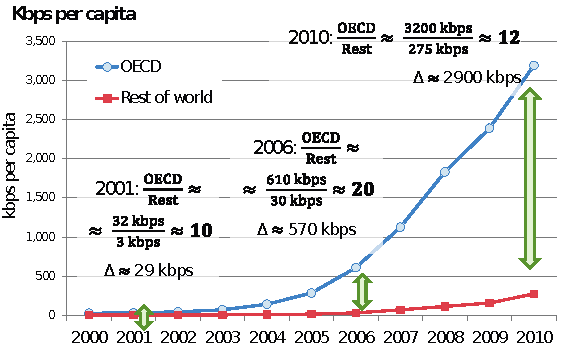
\includegraphics[width=\textwidth]{figures/kbpspercapita.pdf}
\caption[Telecom capacity per capita]{Kilobytes per second optimally compressed telecom capacity per capita \cite{SIGN:SIGN584}. Telecom includes fixed and mobile, telephony and internet. \label{fig:growth}}
\end{figure}

Figure \ref{fig:growth} illustrates the growth of telecom capacity over the years per capita. A distinction has been made by The Organization for Economic Co-operation and Development (OECD), which is an international economic organization of 34 countries founded in 1961 in order to stimulate economic progress and world trade. OECD countries are in general well developed countries of which the GDP per capita is in the highest quartile. The figure shows that while in 2001 the average inhabitant of the developed OECD countries had an installed telecommunication capacity of 32kbps, in 2010 the access capacity of an individual inhabitant had already multiplied by a factor of 100 to 3200kbps \cite{SIGN:SIGN584}.

Besides the volume, data is shifting from static sets to a continuously changing nature \cite{1558609016}. The handling of such massive amounts of dynamic data is known as `big data', which comprises datasets whose sizes are far beyond the ability of commonly used software tools to capture, curate, manage, and process within a tolerable time frame \cite{bigdata}. Many definitions of big data exist, as we follow the definition \cite{Hashem201598}: `Big data is a set of techniques and technologies that require new forms of integration to uncover large hidden values from large datasets that are diverse, complex and of a massive scale'. To obtain insights from large amounts of data, different tooling is required. For example, most relational database management systems and desktop statistics are not up to the task, instead we need `massively parallel software running on tens, hundreds, or even thousands of servers' to process the data \cite{Jacobs:2009:PBD:1536616.1536632}.

The process of extracting valuable knowledge from the large and complex amounts data is known as data mining, defined as `the non-trivial extraction of implicit, formerly unidentified and potentially constructive information from data in databases' \cite{Zaiane99introductionto,Kantardzic:2002:DMC:581837}. The goal of data mining is to mine the so-called golden nuggets from the mountain of data \cite{1347303}. The golden-nuggets are observations which provide knowledge about the data. Outlier detection, a subdivision of Knowledge Discovery and Data mining (KDD) differs in the sense that it detects data which shows behavior that differs from the rest of the data, and which might possibly be a so-called golden nugget \cite{Chandola:2009:ADS:1541880.1541882}.

Outlier detection has been studied by the statistical community as early as the $19^{\text{th}}$ century to highlight noisy data from scientific data sets \cite{14786448708628471}. For example, for normally distributed data, the observations which lie outside three times the standard deviation are considered outliers \cite{9783540262565}. Another commonly used method is based on statistical models, where a wide range of tests are used to find the observations which do not fit the model \cite{barnett1994outliers}. Such parametric models are not always suitable for general purpose outlier detection as it is not always clear which distribution the data follows. Recent outlier detection algorithms observe the local neighbouring observations and determine the outlierness based on the differences of the local neighbourhood.

The term `anomaly' or `outlier' is an ambiguous term, therefore a definition is in place. First, an outlier, sometimes referred to as an anomaly, exception, novelty, fault or error is defined as;
\begin{itemize}
  \item ``An observation which deviates so much from other observations as to arouse suspicions that it was generated by a different mechanism.'' \cite{Enderlein1987}
  \item ``An outlying observation, or ‘outlier,’ is one that appears to deviate markedly from other members of the observation in which it occurs.'' \cite{Grubbs1969}
  \item ``An observation (or subset of observations) which appears to be inconsistent with the remainder of that set of data.'' \cite{barnett1994outliers}
  \item ``An outlier is a data point that deviates quantitatively from the majority of the data points, according to an outlier-selection algorithm.'' \cite{outlierselection}
\end{itemize}

We follow the last definition, as we believe it is of importance to prove quantitatively that the data point is different from the majority of the set. Outliers may be `surprising veridical data', as belonging to class $\mathcal{A}$, but actually situated inside class $\mathcal{B}$, so the true classification of the point is surprising to the observer \cite{John95robustdecision}. Outlier detection analysis in big data may lead to new discoveries in databases, but an outlier can also be noise---a faulty sensor, for example. Finding aberrant or disturbing observations in large collections is valuable and might be a subject for further investigation. Outlier detection has a variety of applications, among which:

\begin{description}
  \item[Log analysis] Applying outlier-detection on log files helps to uncover issues with the hard- or software of a server. Applying it to network or server logs can unveil possible hacking attempts. 
  \item[Financial transactions] In recent years, outlier detection within the financial world has drawn considerable attention in research \cite{Kanhere2014}. By the use of outlier detection on credit-card transactions it is possible to indicate credit card fraud or identity theft \cite{618940}.
  \item[Sensor monitoring] As sensors are becoming cheaper and more integrated in our world, outlier detection can be used to monitor the data and identify faulty sensors \cite{Fujimaki:2005:ASA:1081870.1081917}.
  \item[Noise removal] Outlier detection is often used for the preprocessing of data in order to clear impurities and discard mislabeled instances \cite{Brodley96identifyingand}. For example, before training a supervised model, the outliers are removed from the training-dataset, thus removing possible noisy observations or mislabeled data \cite{63857}.
  \item[Novelty detection] Novelty detection is related to outlier detection as a novelty is most likely different from the known data. An example application is the detection of new topics of discussion on social media \cite{Markou20032481,Markou20032499,SPC3:SPC3353}.
  \item[Quality control] ``Outlier detection is a critical task in many safety critical environments as the outlier indicates abnormal running conditions from which significant performance degradation may well result, such as an aircraft engine rotation defect or a flow problem in a pipeline. An outlier can denote an anomalous object in an image such as a land mine. An outlier may pinpoint an intruder inside a system with malicious intentions so rapid detection is essential. Outlier detection can detect a fault on a factory production line by constantly monitoring specific features of the products and comparing the real-time data with either the features of normal products or those for faults'' \cite{6416666}.
\end{description}

Introducing outlier detection into the realm of web-scale computing will introduce requirements on the architecture, data-storage and deployment of the application. The data center has become a major computing platform, powering not only internet services, but also a growing number of scientific and enterprise applications \cite{Zaharia:2011:DNO:2170444.2170461}. By deploying the outlier detection systems on a cloud architecture allows the system to scale its capacity according to the current needs. For example, when an outlier detection algorithm listens to a stream of financial transactions, it needs to scale up at Christmas due the increase of workload, and can be scaled down every Sunday freeing up resources which can be used by other services such as reporting.

It is difficult to determine if an observations is a true anomaly, but when marked as an outlier by the algorithm, it is probably worth further investigation the observation by a domain expert. Outlier detection is not new, but has not yet been widely implemented in a scalable architecture. From Quintors' perspective a shift in requirements becoming more evident each day. As the data changes faster, classical data warehousing/mining is not up to the job and a shift has to made to the realm of real-time processing \cite{1640284}. By providing real-time tactical support to drive actions that react to events as they occur. This requires shifting from batch-processing jobs to real-time processing. By real-time processing we refer to soft real-time whereby the added value of the results produced by a task decreases over time after the deadline expires \cite{259423}. The deadline is considered the expiration of the time span in which the result is expected.

\section{Research questions \label{sec1-researchquestions}}

The main focus of the thesis is on outlier detection within a scalable architecture, most standard outlier-detection algorithms do not consider an implementation on a web-scale level. Therefore the goal of this thesis is providing a scalable implementation which can be used in industry to apply outlier detection to very large data sets.

The research question and its sub-questions presented next will be supported, referred to and addressed throughout the thesis. By breaking the main question down into several sub-questions the different concerns can be isolated and addressed separately.

\begin{research-question} 
How to scale a general purpose outlier detection algorithms to a web-scale level. \label{req1}
\end{research-question}   

Outlier detection is part of the domain of Knowledge Discovery and Data mining (KDD). Most implementations are not developed with scalability in mind, but solely on the method to uncover outliers from the set of observations. Therefore the first question is to determine which algorithms can potentially benefit from a parallel implementation.

\begin{research-sub-question} 
Which general-purpose outlier detection algorithms can potentially be scaled out. \label{sub-req1}
\end{research-sub-question}

Scaling an algorithm out, or sometimes referred as scaling horizontally, is distributing the workload of the algorithm across different machines which will act as a single logical unit. The different methods of outlier detection needs examined to determine if it can be converted into a so called `embarrassingly parallel workload'. This requires the algorithm to be able to separate the problem into a number of parallel tasks which can be scheduled on a cluster of distributed machines.

\begin{research-sub-question} 
Which computational engines are appropriate for distributed outlier detection. \label{sub-req2}
\end{research-sub-question}

Recent years a variety of computational engines have been developed for developing distributed applications, mostly based on the MapReduce model \cite{Dean:2008:MSD:1327452.1327492}, such as Apache Hadoop\footnote{Apache Hadoop \url{http://wiki.apache.org/hadoop/HadoopMapReduce}}, Apache Spark \cite{Zaharia:2010:SCC:1863103.1863113}. Other frameworks, such as Apache Mahout\footnote{Apache Mahout \url{http://mahout.apache.org/}}, provide additional algorithms which run on top of computational engines. An overview will be given of available computational engines and their characteristics.


\begin{research-sub-question} 
How to adapt the algorithm to work with streams of data, rather than a static set. \label{sub-req3}
\end{research-sub-question}

Rather than mining outliers from a static set of data, data comes most of the time as a stream. Example streams are sensor data or transactions which arrive over time. Important to note is that data streams are likely to evolve over time.

\section{Quintor \label{sec1-Quintor}}
Quintor is a leading player in the fields of Agile software development, enterprise Java / .Net technology and mobile development. Since its foundation in the year 2005, Quintor has been growing steadily. From their locations in Groningen and Amersfoort, they provide support to their customers in facing the challenges that large-scale enterprise projects entail. Quintor has a software factory at its disposal, from where in-house projects are carried out. 

To our enterprise customers, Quintor provides services in the field of software development processes (Agile/Scrum), information analysis, software integration processes, automated testing, software development and enterprise architecture. Quintor provides full Agile development teams consisting of analysts, architects and developers.

From Quintors' perspective the area of big-data is experiencing a tremendous growth and companies are looking for ways to extract knowledge from their data to obtain strategic insights.
